\section{Understanding Kiva website and Dataset}

\begin{itemize}
	\item Describe what user can do on the website: search for Projects, Auto-lending setup
	\item Describe how to get the data using GraphQL, Crawling method
	\item Describe data schema: fields that we can get, the meaning of each fields
	\item Describe preprocessing steps with the data
	      \begin{itemize}
		      \item Steps: accelerated loading, forming the big table, removing unwanted tags, remove anonymous Lenders, handle duplicates\dots
		      \item Forming the tri-partite graph: Lenders-Projects-Tags
		      \item Mention that we have to use CuDF for accelerated data handling
	      \end{itemize}
\end{itemize}

In this section, we will describe the Kiva website and the dataset that we use in this thesis.
We will also describe the preprocessing steps that we have to do with the dataset.

While there are many crowdfunding platforms,
we specifically choose Kiva because of its transparancy and the avalability of the data for public access.

\subsection{Kiva website}

To understand the data that the platform provides, we have to understand the interface that the platform provides to its users.
Like other platform, Kiva has a website where users can login and interact with the platform.
To understand the data that the platform provides and to extract meaningfull insight from the data,
we have to understand the interface that the platform provides to its users.

Any website interface is designed to make users interact with it in a pre-defined way.
In Kiva, we belived that the most function that users can do is to search for projects that they want to fund.
Or they can setup an Auto-Lending program, which will automatically fund projects that fit their criteria.


\begin{figure}[H]
	\centering
	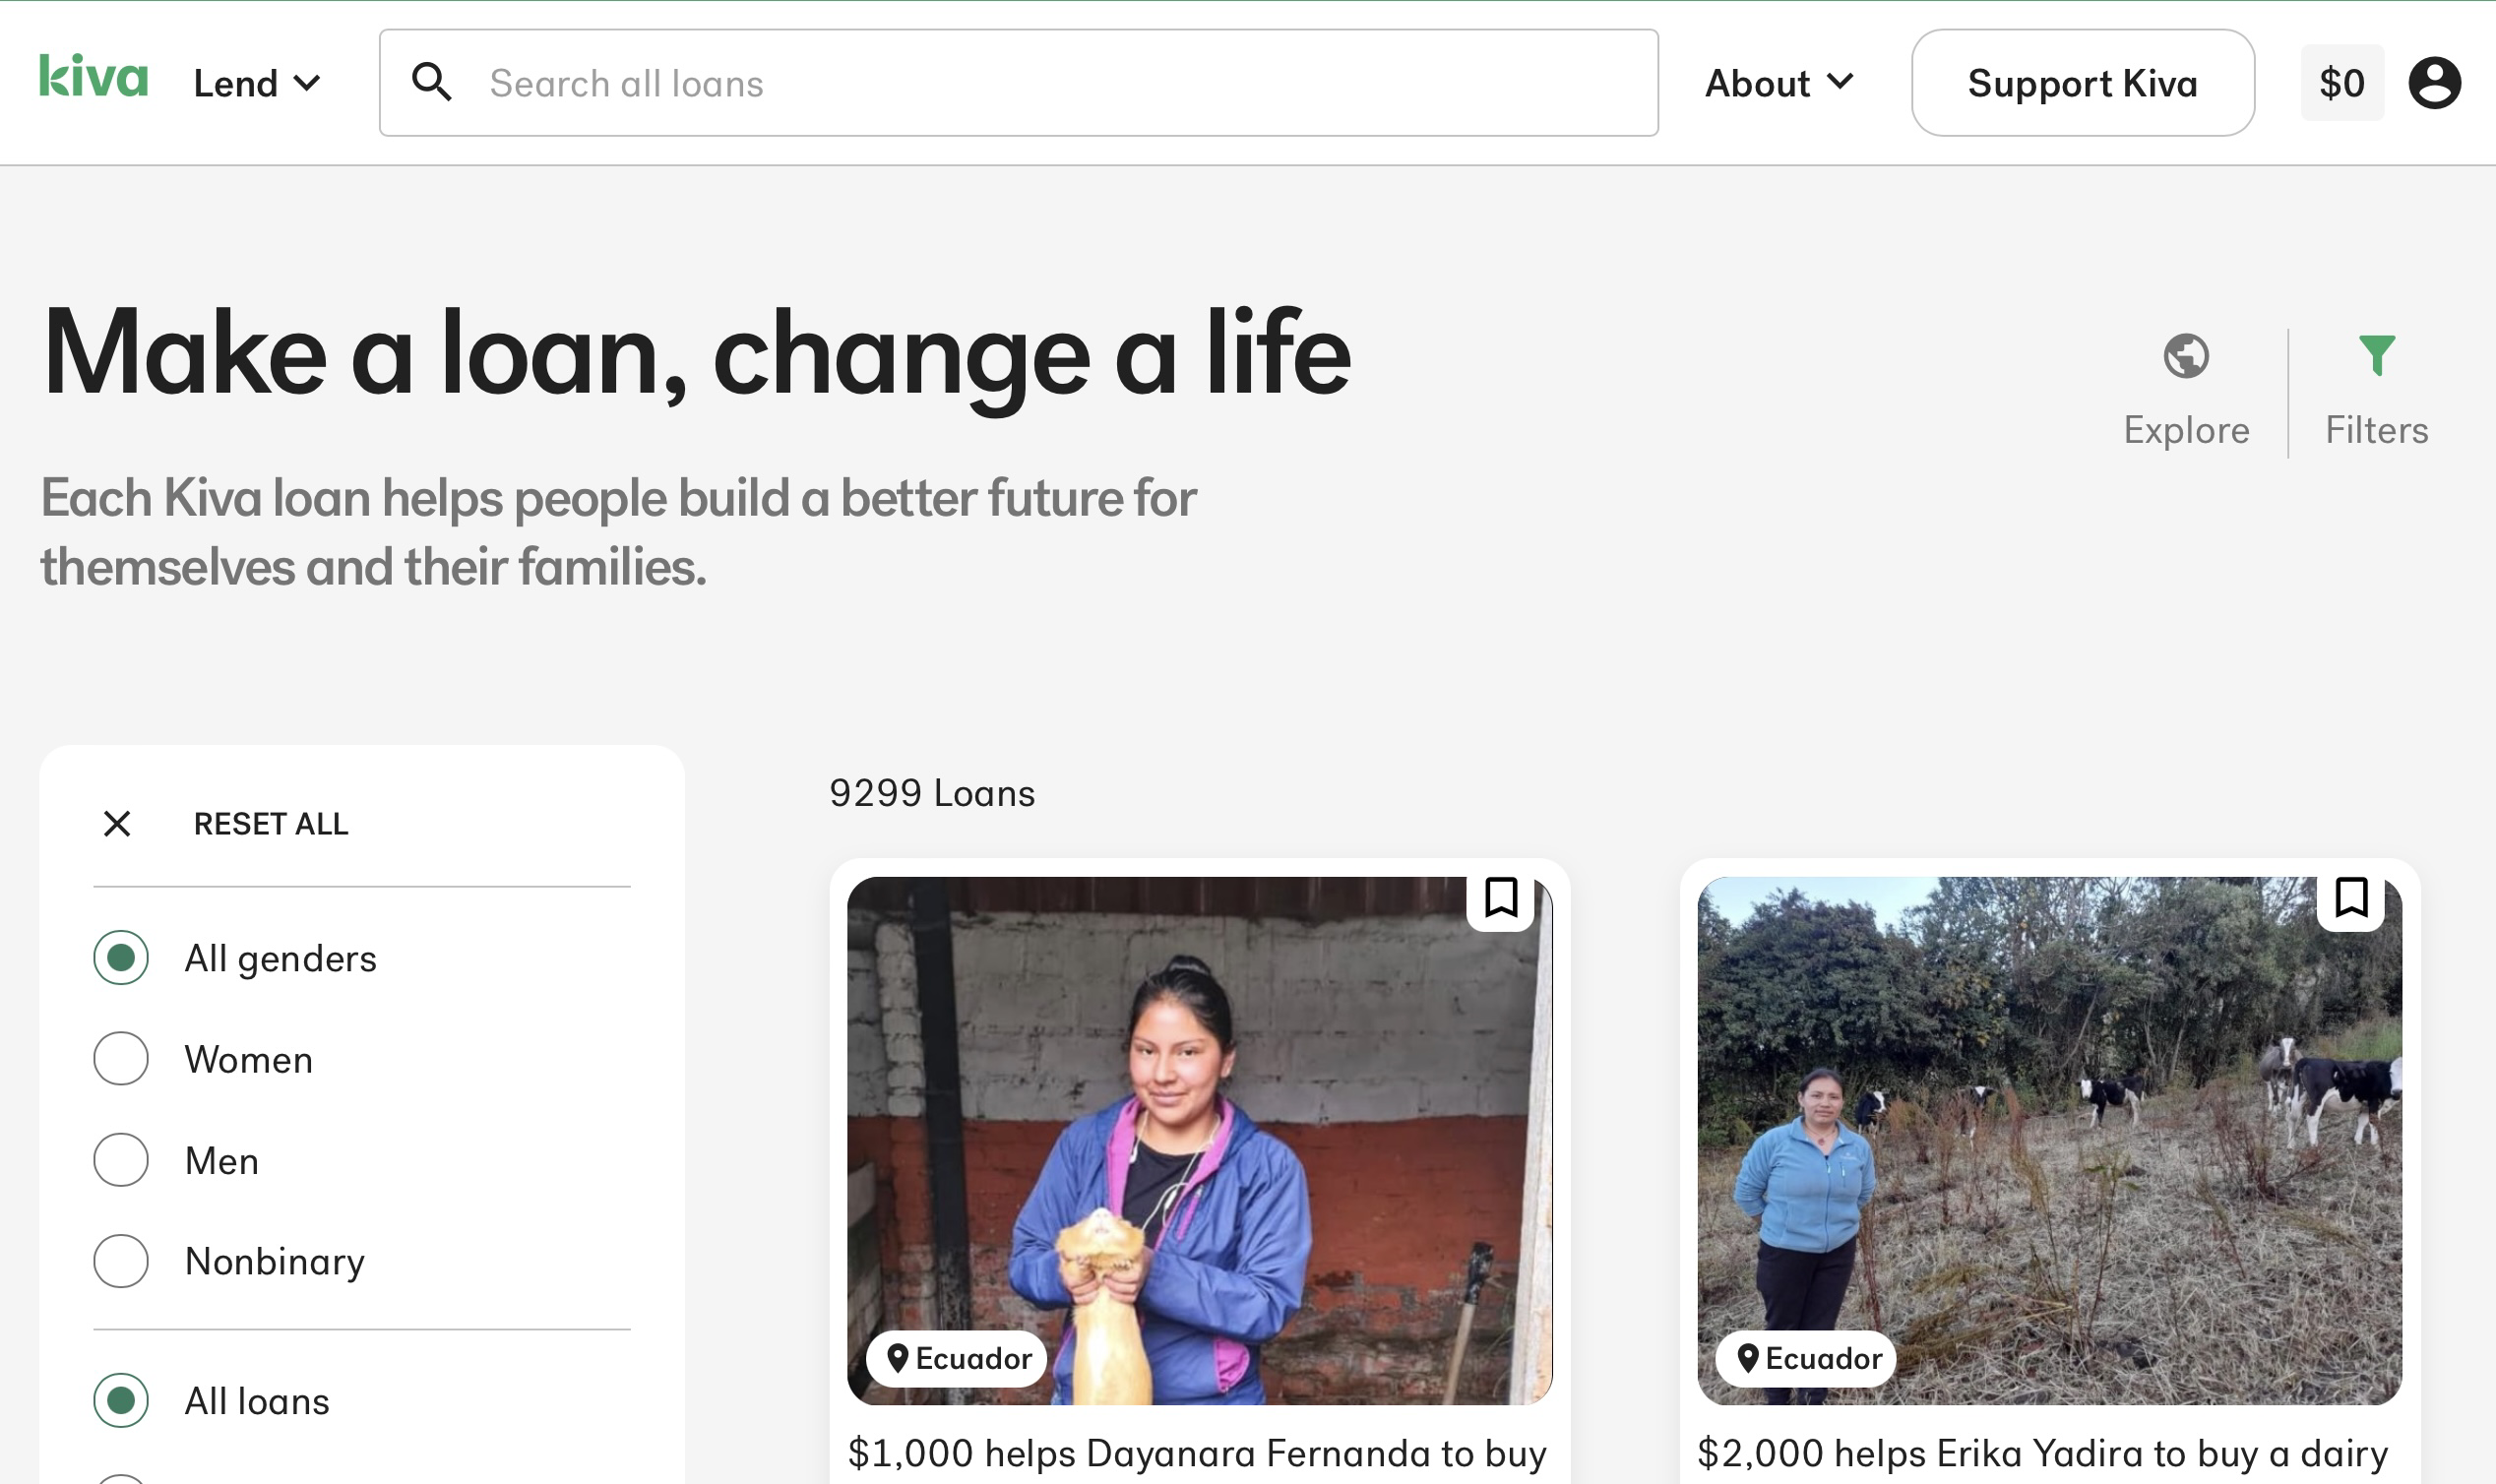
\includegraphics[width=0.8\textwidth]{images/kiva-browse-project.png}
	\caption{Kiva website interface for browsing projects \cite{kiva-browse}}
	\label{fig:kiva-browser-project}
\end{figure}

It is important to know what Lenders can do when looking for his or her interested project.
Table \ref{tab:browser-criteria} shows the criteria that Lenders can use to filter the projects.
Later in the thesis, we will see that these criteria is not very align with the public data that the platform provide.
For example in the data, we could see some Tags that did not appear in the Tags list in the website.
We will consider these criteria as the gold standard for processing the data.

\begin{table}[H]
	\centering
	\resizebox{\textwidth}{!}{%
		\begin{tabular}{|l|l|l|l|}
			\hline
			   & Options                       & Type            & Choices                                                                                                                 \\
			\hline
			1  & Gender of the borrower button & Single Choice   & Woman or Men or Nonbinary                                                                                               \\
			2  & Filter by type of Loan        & Single Choice   & Individual or Group                                                                                                     \\
			3  & Search by keyword             & Text            & Put any keyword to search in the stories of Projects                                                                    \\
			4  & Sort Order                    & Single Choice   & Amount: High to Low, Amount left, Amount: Low to High, Ending soon, Most recent, Trending now, Loan Length, Recommended \\
			5  & Location                      & Multiple choice & Choose from a list of countries                                                                                         \\
			6  & Sector                        & Multiple choice & Choose from a list of sectors                                                                                           \\
			7  & Attribute                     & Multiple choice & Choose from a list of attributes                                                                                        \\
			8  & Tags                          & Multiple choice & Choose from a list of tags                                                                                              \\
			9  & Loan Length                   & Single Choice   & All loans, 8 month or less, 16 months or less, 2 years or less, 2 years or more                                         \\
			10 & Loan Distribution             & Single Choice   & All loans, Parter, Direct                                                                                               \\
			11 & Partner Info                  & Text            & Search by Partner name                                                                                                  \\
			12 & Risk Rating                   & Range           & From 1 to 5                                                                                                             \\
			13 & Default Rate                  & Range           & From 0\% to 100\%                                                                                                       \\
			14 & Profitability                 & Range           & From -160\% to 90\%                                                                                                     \\
			\hline
		\end{tabular}%
	}
	\caption{Project filtering options on Kiva's website \cite{kiva-browse}}
	\label{tab:browser-criteria}
\end{table}

Perhaps the most unique feature of Kiva is the Auto-Lending program.
In the program, Lenders can setup criterias for future projects that they want to fund.
When a new project is created, the platform will automatically fund the project if it fits the criterias.
Figure \ref{fig:auto-lend-setup} shows the interface for setting up the Auto-Lending program.

\begin{figure}[H]
	\centering
	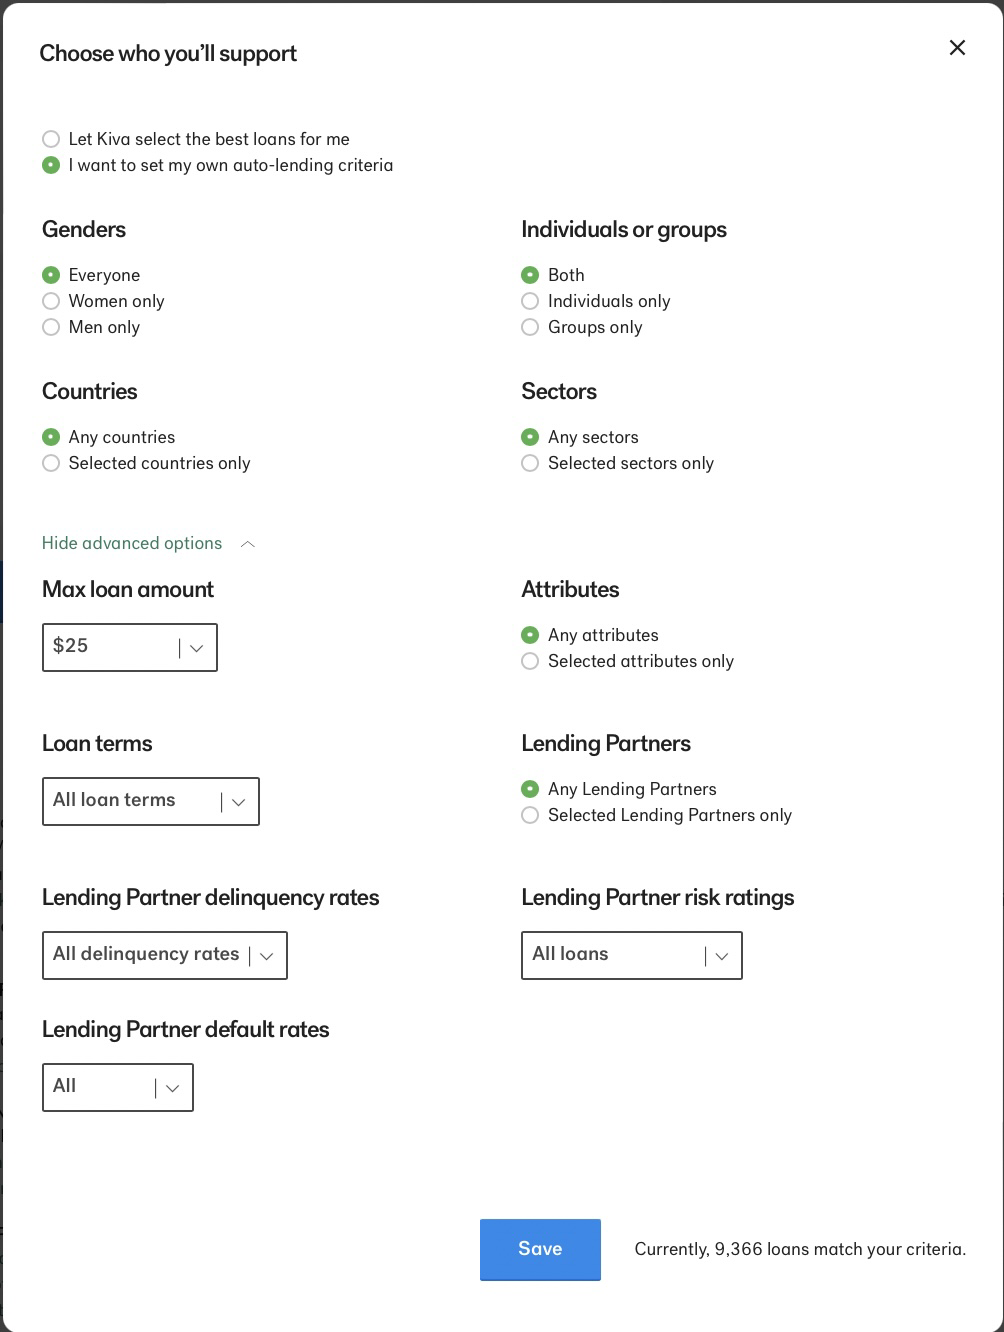
\includegraphics[width=0.8\textwidth]{images/auto-lend-setup.png}
	\caption{Auto-Lending setup interface \cite{kiva-autolend2}}
	\label{fig:auto-lend-setup}
\end{figure}

Users can "Let Kiva select the best loans for me" or "I want to set my own auto-lending criteria".
We do not have any information about how the platform select the best loans for users.
So we will focus on the second option.
We can see that the criterias are very similar to the criterias that users can use to search for projects.

\subsection{Kiva Data Access}

In order to access the data provided by Kiva, we utilize the GraphQL API.
Kiva has made their data available through this API, allowing developers to query and retrieve specific information from the platform.
This is perhap unique to Kiva, as most other crowdfunding platforms do not provide such access to their data.
It is also note that Kiva also provides a public dataset through their so called "Data Snapshot".
However, this function is appearantly not working at the time of writing.
There also another way to get the data from kiva website, which is through Web Crawling.
By analysis the website interface and the network traffic, we can get the data that the website use to display the information.
This approach is although popular, but it is not very reliable because the website can change its interface at any time.
In this thesis, we will focus on the GraphQL API.

GraphQL is a query language for APIs that provides a flexible and efficient way to request and manipulate data.
It allows us to specify the exact data we need and retrieve it in a single request, reducing the amount of network traffic and improving performance.
By leveraging the GraphQL API, we can easily access various data points such as borrower information, loan details, lender statistics, and more.
This enables us to perform in-depth analysis and gain valuable insights from the Kiva dataset.
The availability of Kiva's data through GraphQL provides us with a powerful tool to explore and analyze the platform's data in a convenient and efficient manner.

There are two noteworthy points about the GraphQL API.
The first is through the \textit{introspection} \cite{graphql-introspection} feature of GraphQL,
we could have the information of what queries that the platform supports,
as long as with the data schema.
The second is that we can ultilize the GraphQL API to get the data in a batched manner.
Usually the platform will limit the number of requests that a user can make to the API.
But if we use some Web Crawling techniques, we can manage to get all the data that avaliable in the API.

Kiva GraphQL API can be found publicly at \url{https://api.kivaws.org/graphql}.
One can connect to the URI with any compatible GraphQL client.
On top of that, kiva also use \textit{GraphQLi}, a web interface for easy try the GraphQL queries.
\ref{fig:grapqli} is the screenshot of the web interface.
We use the interface to introspection the data schema and to try out some queries before actually implementing them in the code.

\begin{figure}[H]
	\centering
	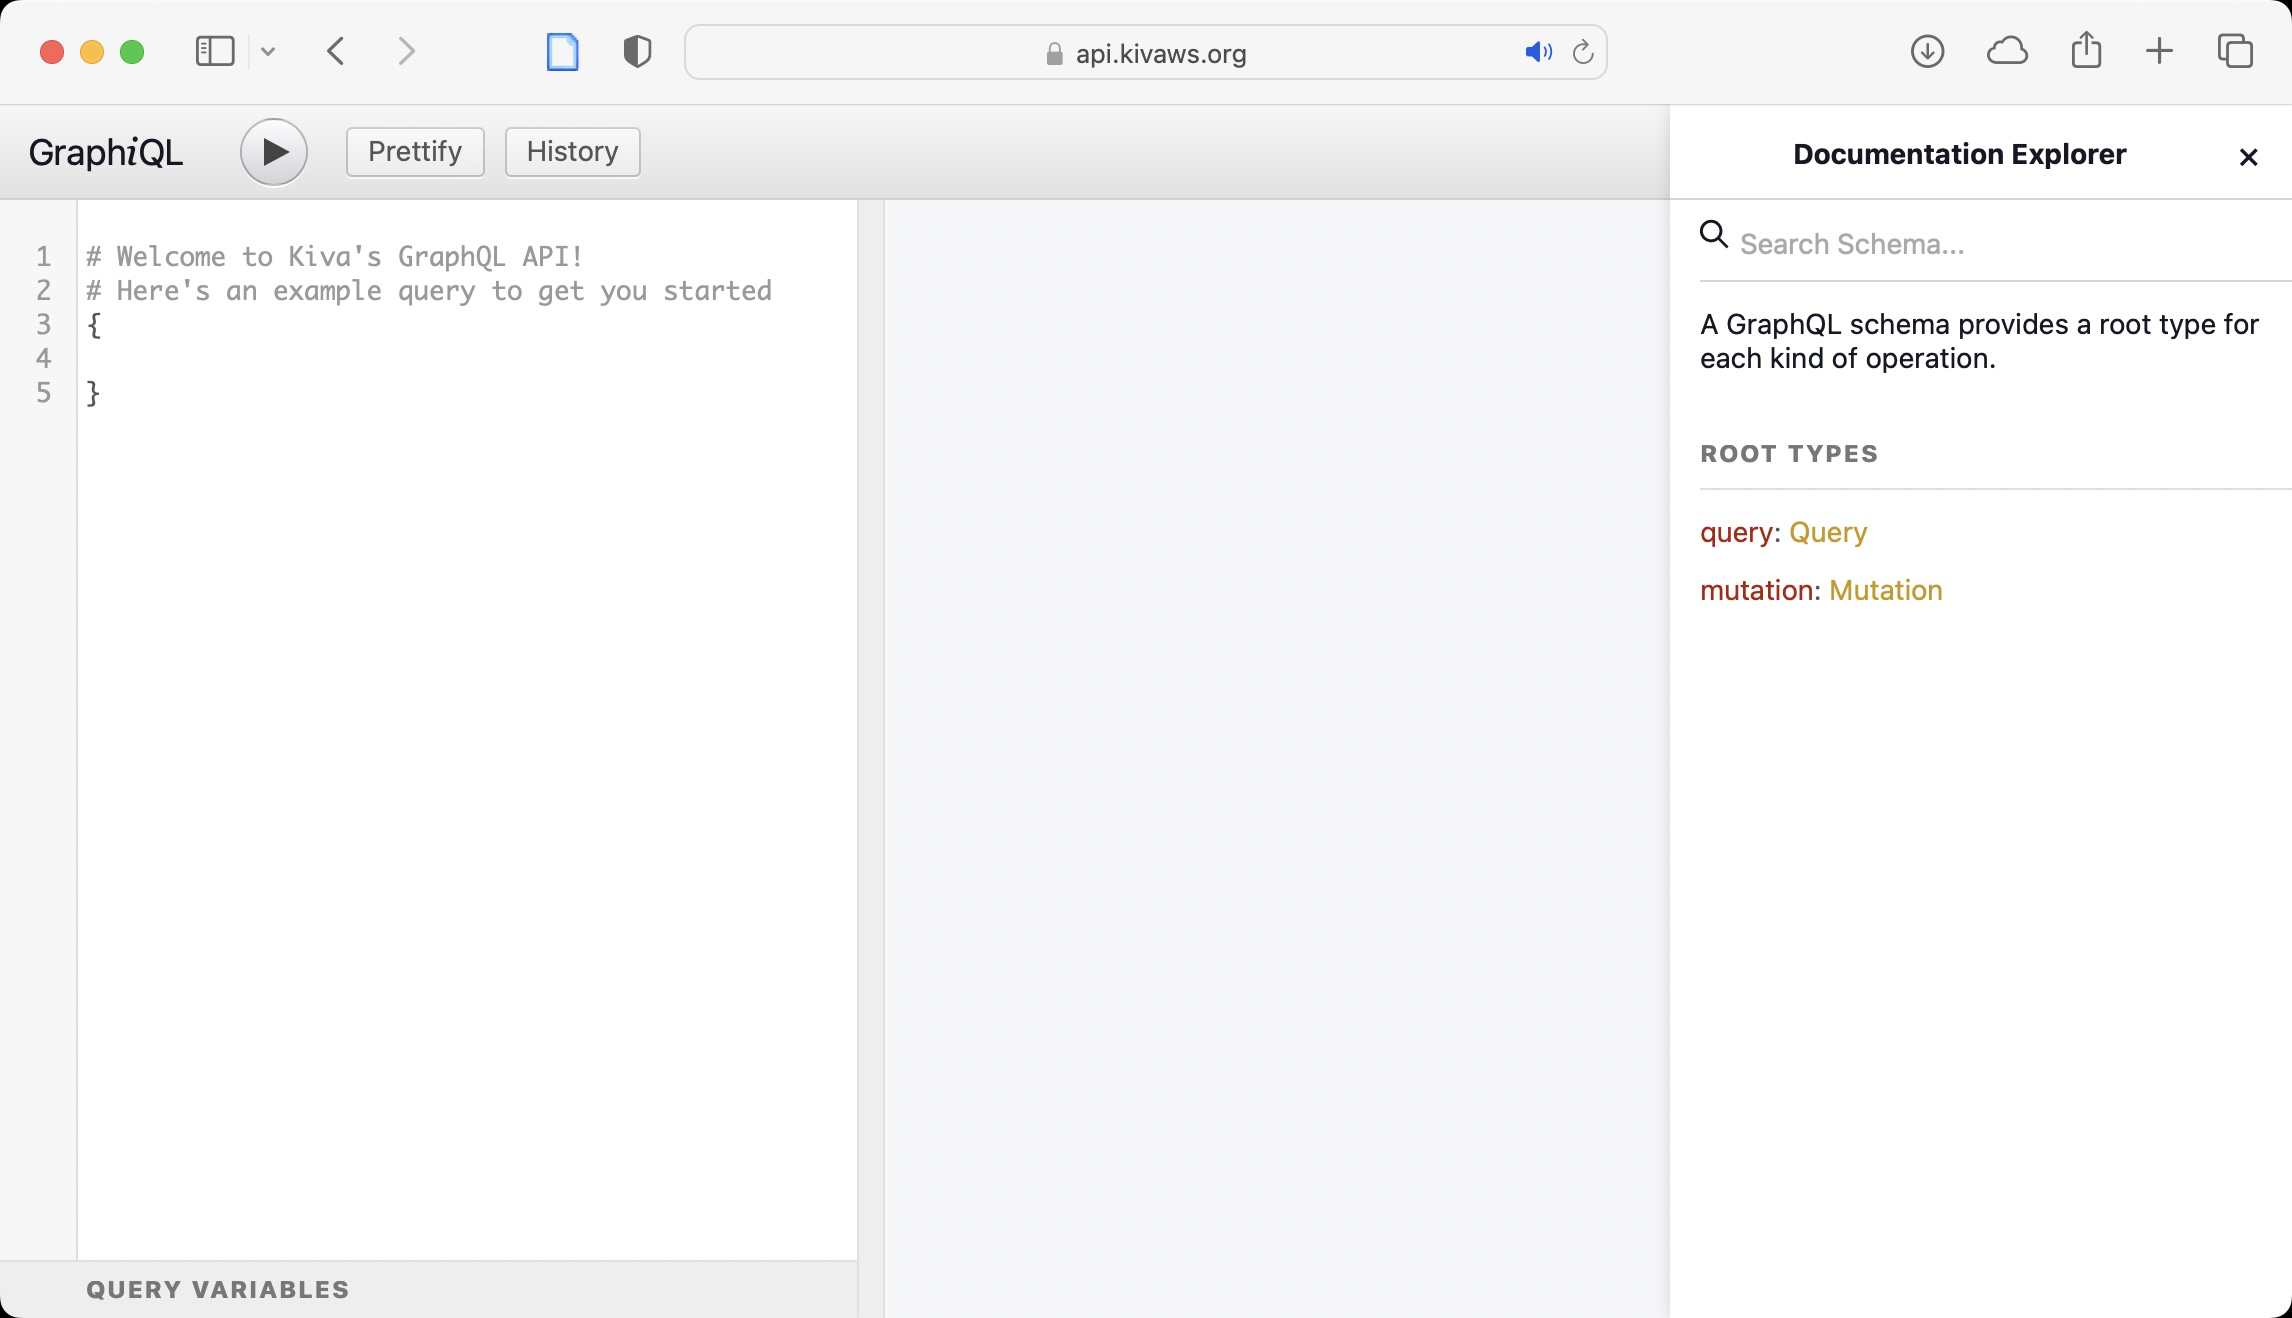
\includegraphics[width=0.8\textwidth]{images/grapqli.png}
	\caption{GraphQLi interface of Kiva GraphQL API}
	\label{fig:grapqli}
\end{figure}

For example, we could try the query for getting basic stats of kiva like following Figure \ref{fig:graphqli-example}.
One can use the Docs side bar (the right side bar) to discover what is the data that the API offer.
A basic knowledge about GraphQL would be helpful to discover the data schema more easily.

\begin{figure}[H]
	\centering
	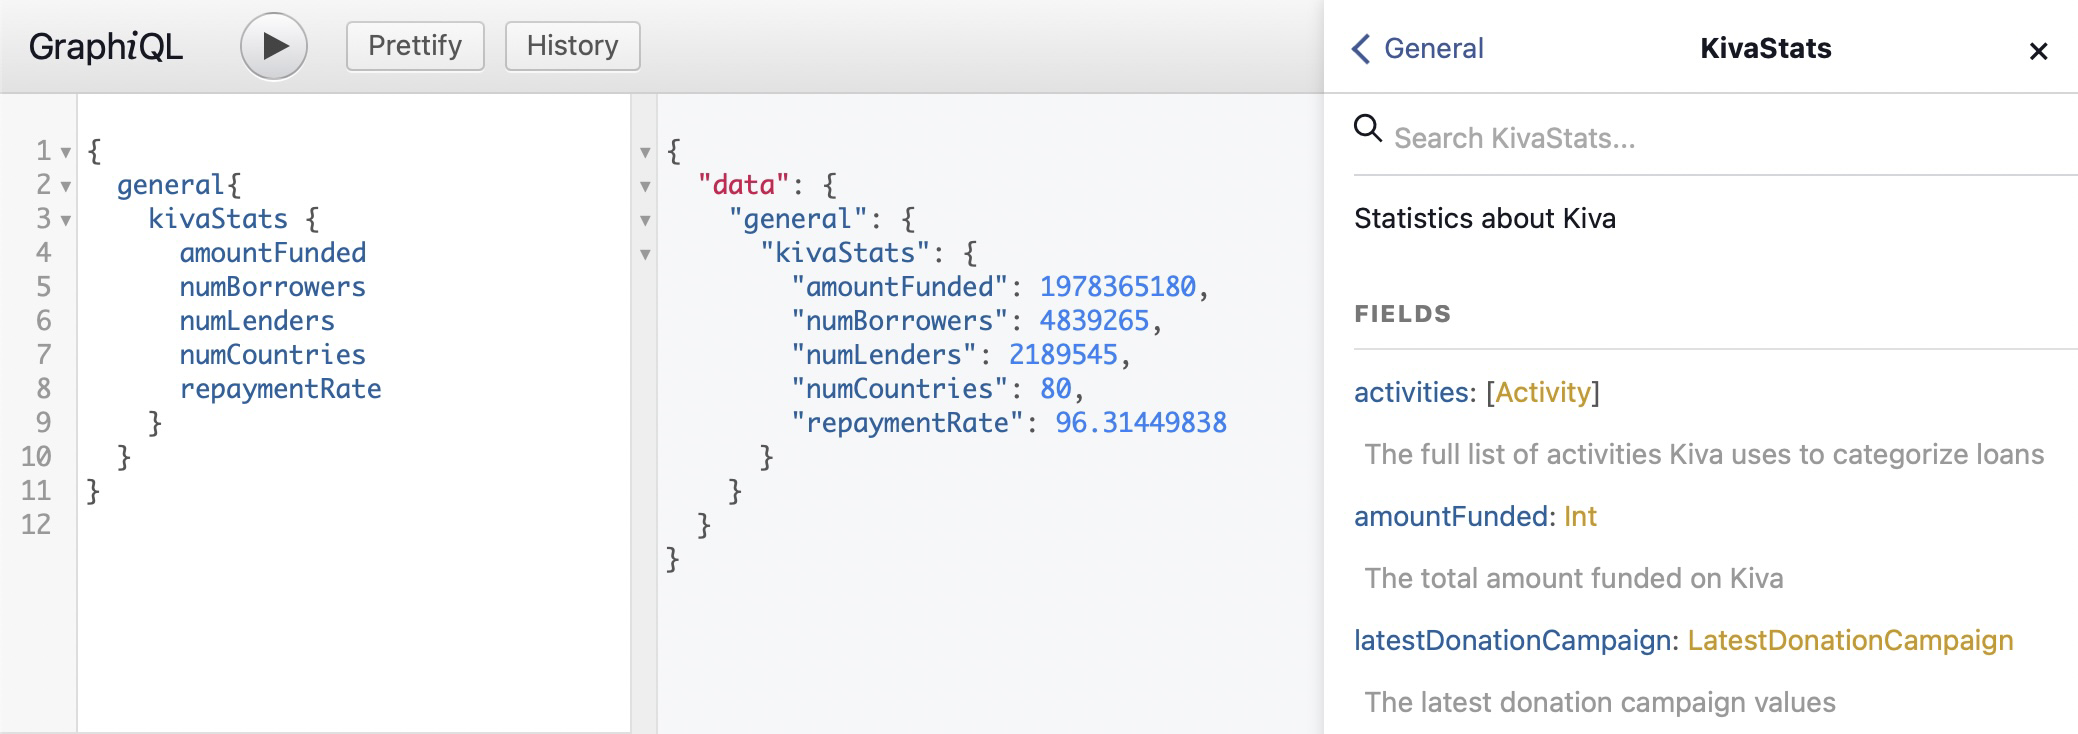
\includegraphics[width=0.8\textwidth]{images/graphqli-example.png}
	\caption{Example using GraphQLi interface of Kiva GraphQL API \cite{graphqli-example}}
	\label{fig:graphqli-example}
\end{figure}


Before begining to query the data, we have to understand the data schema to know what data that we can get.


\begin{figure}[H]
	\centering
	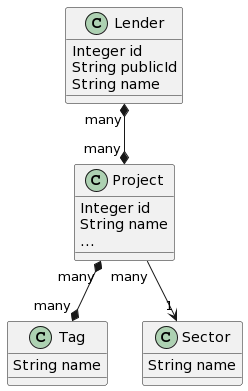
\includegraphics[width=0.25\textwidth]{images/graphuml/dataschema.png}
	\caption{Data schema}
	\label{fig:data-schema}
\end{figure}

The relationship beteen Lender and Project is many-to-many.
Each Project in Kiva can be funded by many Lenders.
And each Lender can fund many Projects.
The relationship between Project and Tag is also many-to-many.
The fields that we could get from each Project is described in Table \ref{tab:appendix-fields-meaning}.
The example data that we get from the API is shown in Table \ref{tab:appendix-example-data}.
We have to note that, in the APIs, kiva use the term "Loan" to indicate a single project.
We found it rather misunderstanding to use "Loan", so we try our best to use "Project" to avoid those misleading.
In this thesis, if a "Loan" appear (with the letter L in capital), one can understand the meaning is a "Project".

Recall that when browse and search for Project in the kiva website,
users can filter Projects by Sectors, Activities, Attributes, Tags.
The API document provide a good definition for some of those terms.

\textbf{\Gls{sector}}

From the API documentation, we have the definition of Sector as, quoted:
"A sector is a broad category for a loan, e.g. Agriculture, Arts, Clothing. Sectors are subdivided further by activities."
We take a step further to get all the possible Sectors that the platform support,
this can be done using the following GraphQL query:

\begin{lstlisting}
    {
        lend {
            sector {
                id
                name
            }
        }
    }
\end{lstlisting}

The result is shown in Table \ref{tab:sector-definition}.

\begin{longtable}[]{@{}rlrl@{}}
	\caption{Definition of Sectors}
	\label{tab:sector-definition}            \\
	\toprule\noalign{}
	id & name           & id & name          \\
	\midrule\noalign{}
	\endhead
	\bottomrule\noalign{}
	\endlastfoot
	1  & Agriculture    & 9  & Arts          \\
	3  & Transportation & 10 & Housing       \\
	4  & Services       & 12 & Food          \\
	5  & Clothing       & 13 & Wholesale     \\
	6  & Health         & 14 & Construction  \\
	7  & Retail         & 15 & Education     \\
	8  & Manufacturing  & 16 & Personal Use  \\
	9  & Arts           & 17 & Entertainment \\
\end{longtable}


\textbf{\Gls{activity}}

"A property of loan which is more descriptive than Sector.
Every activity is within a sector. e.g. the 'Animal Sales' activity is within the 'Agriculture' sector.
Note, some Activities have the same name as their parent Sector."
Quoted from the API documentation.
All the possible Activities can be found using the following GraphQL query:

\begin{lstlisting}
    {
        lend {
            activity {
                id
                name
                }	
        }
    }
\end{lstlisting}

The result is show in Table \ref{tab:appendix-activity-definition}.

\textbf{\Gls{tag}}

The API give the definition of Tag as,
quoted: "Loan properties which are attributed by lenders"
With the following GraphQL query, we can get all the possible Tags that the platform support.

\begin{lstlisting}
    {
        lend {
            tag {
                id, # Unique identifier for this tag
                name, # The name of the tag
                vocabularyId # Vocabulary id for the tag type
            }
        }
    }
\end{lstlisting}

The result is shown in Table \ref{tab:appendix-tag-definition}.


Kiva did not provide any documentation about the meaning of the name of Tags,
as well as the meaning of \lstinline|vocabularyId|.
When browsing Project in the website, one could found \textit{Attribute}.
When explore the API, one could also found \textit{Theme}.
There is no documentation on what is Attribute and Theme.
We suppose that Attribute and Theme are the same thing.
But since the meaning of the Attribute and Theme is not clear,
we decided to not use them in our analysis.

Once understand the data schema, we can start crawling the data.
We decided to get all the fields of the Project, as well as the fields of the nested objects.

In order to retrieve all data using the API, we ultilize the \textit{scrappy}\cite{scrappy} framework.
Perhaps the most useful feature of scrappy is that it can automatically bypass the rate limit of the API.
It is common that APIs should have a rate-limit mechanism to prevent users from abusing the API.
While Kiva API is not an exception, it do not provide a clear documentation about the limit.
To overcome this problem, we use scrappy with the option \lstinline|AUTOTHROTTLE_ENABLED = True|.
This option will automatically slow down the request rate when the response time is too long.
This will prevent the API from being abused and also allow us to get all the data in a reasonable time without being blocked.
In our experiment, we found that the API will only give roughly 500-600 Projects per minutes.
At the time of crawling, the platform has approximately 2.5 million Projects.
So it would take roughly 80 hours to get all the data under the ideal circumstances, assuming no error occurs.

There are also two notable decisions that we made when crawling the data.
The first one is the order of the Projects.
Since we get the data in batch, it is of paramount important to maintain a fix order of crawling.
Otherwise, we could end up with duplicate data or, worst, missing data.
In practice, we decided to use the order that the newest Projects are crawled first.
This is because the GraphQL API already support it, and the newest Projects are more likely to be crawled successfully.
The second decision is the format of data storing.
While nowaday, there are advanced data type that can store data and provide reading in a more efficient way,
such as \textit{Parquet}\cite{parquet} or \textit{HDF5}\cite{hdf5}.
But when it comes to crawling data, we would like to have a format that is easy to append new data,
as long as quickly read a part of the data for monitoring the crawling progress.
Those format, while advanced, is binary format, meaning that it is not easy to append new data or read a part of it.
In practice, we decided to go with \textit{JSONL} format.
Each Project will be stored in a single line, and the whole file is a valid JSON file.
This format is easy to append new data, and also easy to read a part of it, and remaining the data structure as defined in the API.

\section{Preprocessing}

After crawling the data, we need to preprocess it before we can use it for analysis.
The goal of preprocessing is to fix any flaw in the data, which can come from the crawling process as well as from the response from API.
We also need to transform the data into a format that is easy to use for analysis.
Note that in the data schema section, we present that the relationship between Lender and Project is many-to-many.
The same is true for the relationship between Project and Tags.
Other relationships (other fields) of Project are one-to-many.

Because of that, and with another reason is that we want to maintain a single source of truth for all the analysis,
we would like to create a long-table format for the data.
In this format, each row has three main parts: Lender part, Project part, and Tag part.
The Lender part contains all the information about the Lender which related to the Project.
The Project part contains all the information about the Project.
The Tag part is just a single column that contains the Tag name.


\begin{figure}[H]
	\centering
	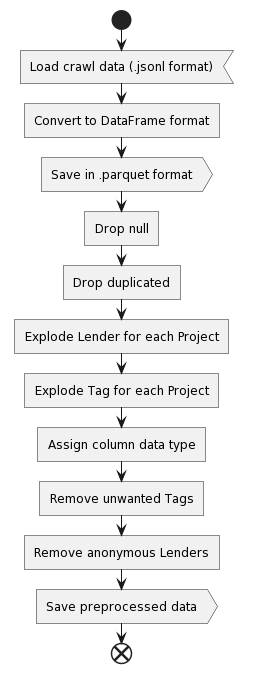
\includegraphics[width=0.2\textwidth]{images/graphuml/preprocessing.png}
	\caption{Preprocessing steps}
	\label{fig:preprocessing}
\end{figure}

Figure \ref{fig:preprocessing} shows the steps of preprocessing.
We will explains each step in detail in the following sections.
But before it, we would like to list the tools that we use for the task.
We use Python as the language of choice.
When it comes to process data in Python, perhap the most popular library is \textit{pandas}\cite{pandas}.
We took a step further and use \textit{cuDF}\cite{cudf} library, which is a GPU-accelerated version of pandas.
The reason for that is because we would like to have a fast processing time.
So we can quickly iterate over the preprocessing steps.
Meaning that we can try many different preprocessing steps and choose the one most suitable for our analysis.
We also use \textit{Dask}\cite{dask} library to handle bigger-than-memory data.
This is because at first, we do not came up with a good preprocessing pipeline.
We could easily have to process the amount of data that is too large for a GPU to handle.
We use Dask to use multiple GPUs to be able to process the whole dataset.
Although we do not use Dask in the final pipeline, we still cite it here because it is a very useful tool.
In the future works, when the data is even larger than in this thesis, one might found it helpful to use Dask.

The preprocessing pipeline begin with loading the crawled data.
Because the preprocessing steps are not appearantly clear.
We need to explore the data to find out what are the problems.
Hence, it is always a good practice to be able to load the crawled data quickly.
The first things, we use pandas to load the whole crawled data (in \lstinline|.jsonl| format) to memory.
This is possible because the raw data file is roughly 9GB, which is not too large for modern computer.
Right after that, we save the data to a \lstinline|.parquet| file for later use,
because the \lstinline|.parquet| offer much better data compression as well as faster loading time.

Next, two basic preprocessing steps that perhaps will always be done is to check for missing values and duplicated values.
In our case, the missing values and duplicated values are caused by the way that API offer data for us.
In the long duration time of crawling, it is possible that the data in the API will change.
Perhap some new Projects could be add to the platform.
But we decided that, the number of changed is not important for our analysis because the number of changed is small compared to the total number of Projects.
We remove rows that contains all null values.
Then we remove duplicated rows, consider the "id" (a.k.a "project\_id") field as the key.

Look carefully at the example row provided in \ref{tab:appendix-example-data},
we can see that each Projects could have a List of Lenders, and a List of Tags.
Fortunately, the pandas library provide a convenient way to expand those List into multiple rows.
We use the \lstinline|pandas.explode| function to do that.

Next steps, we try to assign a correct data type for each column.
In a nutshell, \lstinline|lender_id|, \lstinline|project_id| should be integer.
Some other fields should be of type \textit{category} because they have a small number of unique values.
Those fields include \lstinline|sector_name|, \lstinline|activity_name|, \lstinline|geocode_country_name|, \lstinline|tag|.
We repeat the assignment with datetime, and float types.

Next steps is to fix the Tag data.
It take us a while to understand the tags data, because some of the tags appear too frequently in the data.
Despite of that, these frequent-tags are not appear in the website interface.
We suppose that these tags are used internally by Kiva to manage the data.
We found that these tags are correspond to the \lstinline|vocabularyId = 1|,
they are \lstinline|volunteer_pick|, \lstinline|volunteer_like|, \lstinline|user_like|, \lstinline|user_favorite|.
We decide to get rid of these tags.

But we suspect that Tags are more complicated than that.
Somes tags are appear that they have special meaning and sounds like they could bring values to users who browsing through the website,
such as \lstinline|#Agriculture| or \lstinline|#Education|, etc.
Despite of that, these tags are not visible to users on the website interfaces.
There are also some tags that even have stranger behavior, such as \lstinline|reserved_crisis_support_loan|.
This tag is not appear in the website interface, nor when we ask the API for all the possible tags.
Yet it appear in the crawl data.

Since the documentation regarding these tags is not exists,
we decided to do our best for understanding what each tags are by looking at some of project for each tags.
We will get rid of the tags the we think is not have any meaning to users and keep the rest.


\todo{Add statistic about the tags and number of Anonymous Lender}

We explore the data, we also found that some Lenders is anonymous.
Though kiva do not provide any documentation about who is anonymous Lender and how they interact with the platform,
we would like to find those Lenders to see if they are minority or majority.

\todo{Add statistic about the tags and number of Anonymous Lender}

The only way to find out if a Lender is anonymous is to look at the \lstinline|lender_name|,
or \lstinline|lender_publicId| fields.
If the lower case of \lstinline|lender_name| is begin with "anonymous",
or the lower case of \lstinline|lender_publicId| is begin with "anon",
then we consider that Lender is anonymous.

\todo{Add comment about remove those Lenders}

After all the above steps, we store the data again in a \lstinline|.parquet| file.
We always keep track of the date of the data, so different version of the data can be easily identify.
We will consider this \lstinline|.parquet| file is a single source of truth for all the analysis.

Well-understanding the data is a crucial step for subsequent analysis.
In the next section, we will provide some statistic about the data.

\section{Basic data statistics}

\begin{comment}
\begin{itemize}
	\item Worldwide statistics
	      \begin{itemize}
		      \item How many projects
		      \item how many lenders
		      \item projects vs country distribution
		      \item successful rate
		      \item \textbf{How long that users stay on the platform}
	      \end{itemize}
	\item Vietnam statistics
	      \begin{itemize}
		      \item How many projects
		      \item \dots
	      \end{itemize}
\end{itemize}
\end{comment}

Recall that for the purpose of the thesis, we would like to find community of Lenders who interest in same type of projects.
Also recall that each project is associated with some fields, such as Sector, Country, Tags, etc.
Through the API, we suppose that these factors could bring good descritive information about the project.
But we have to look carefully at the data to see if it is true.
For instance, if all projects are from the same country, then the country field is not useful.
In this section, we will explore the data to better understand those fields.

\subsection{Geographical Distribution of Projects}

The geographical distribution of Projects is shown in Figure \ref{fig:map-number-project-by-country}.
We can see that although Projects are concentrated in some countries, but they are infact distributed all over the world.
Not only in developing countries like Vietnam, Philippines,
but also developed countries like United States.
It is also interesting to see that there are no Projects in Euro or in Australia.


\begin{figure}[H]
	\centering
	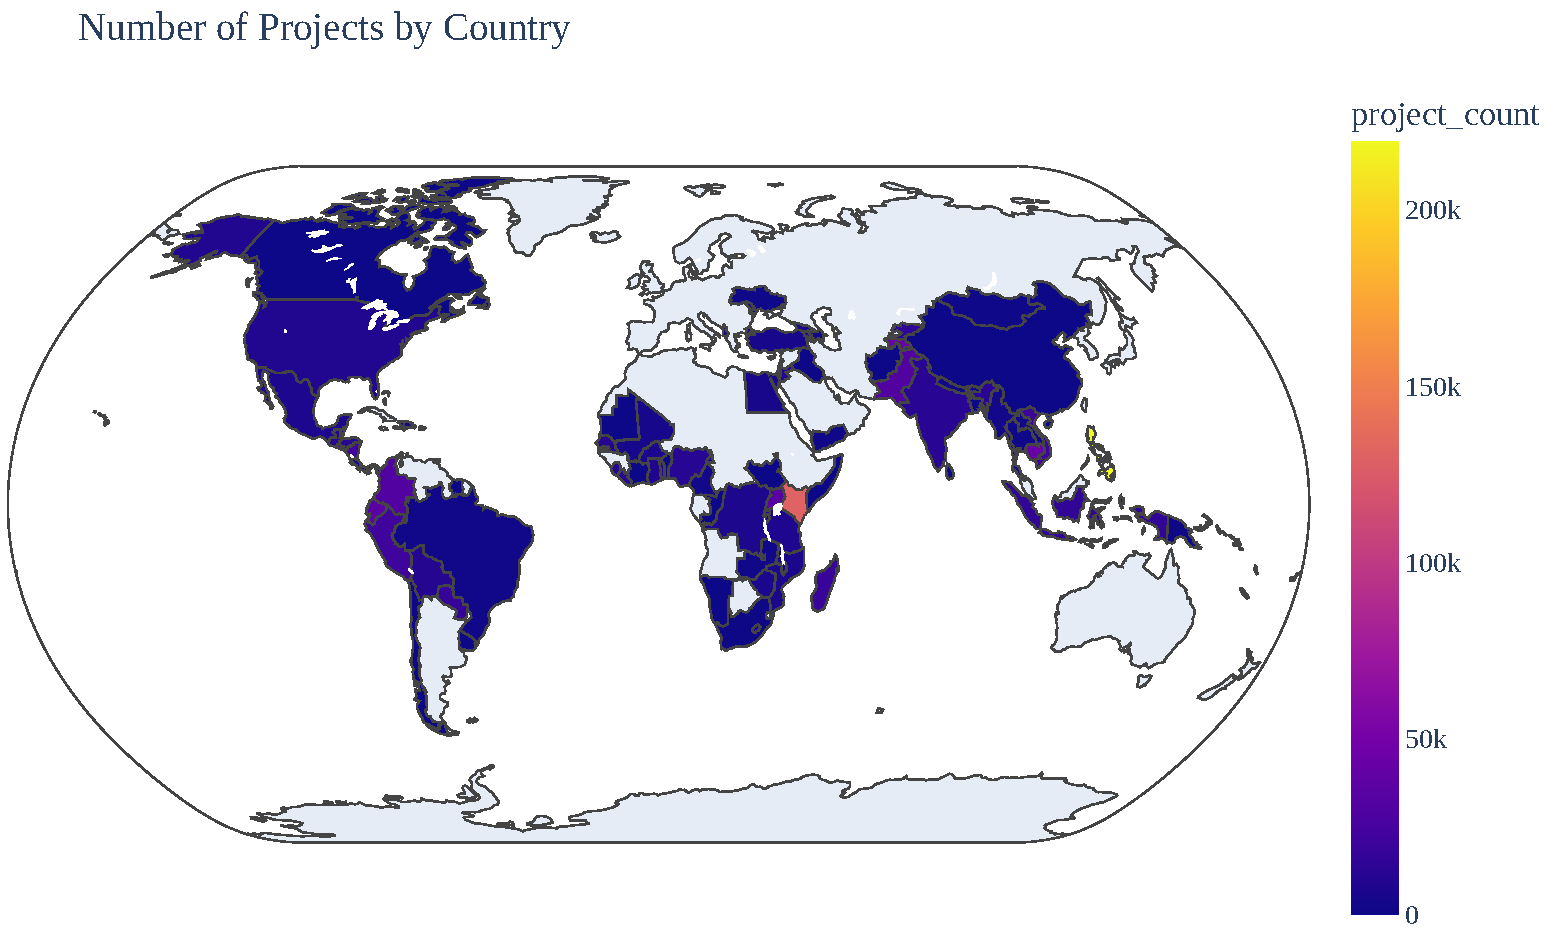
\includegraphics[width=0.95\textwidth]{images/project-vs-country-map.pdf}
	\caption{Geographical Distribution of Projects}
	\label{fig:map-number-project-by-country}
\end{figure}


Look at the georaphical distribution of Projects in Figure \ref{fig:map-number-project-by-country},
we can see that the Projects are from all over the world.
To better visualization, the Figure do not show all the countries.
One can find the detailed information in Table \ref{tab:appendix-project-vs-country}.
Philippines is the country that has the most number of Projects.
The other countries in top 5 are Kenya, El Salvador, Tajikistan, and Cambodia.
The graph also show the average amount of money that each project ask for funding in each country.
We notice that this average is particularly high for the country the right-ending side of the graph.
We suppose that phenomenon is explained by the small number of Projects in those countries,
hence the average is easily affected by the outliers.
But in the left side of the graph, when the number of project is high enough,
notice that the United States has a high average loan amount.
We suppose that this is an interesting finding, and we will explore it in the future works.


\begin{figure}[H]
	\centering
	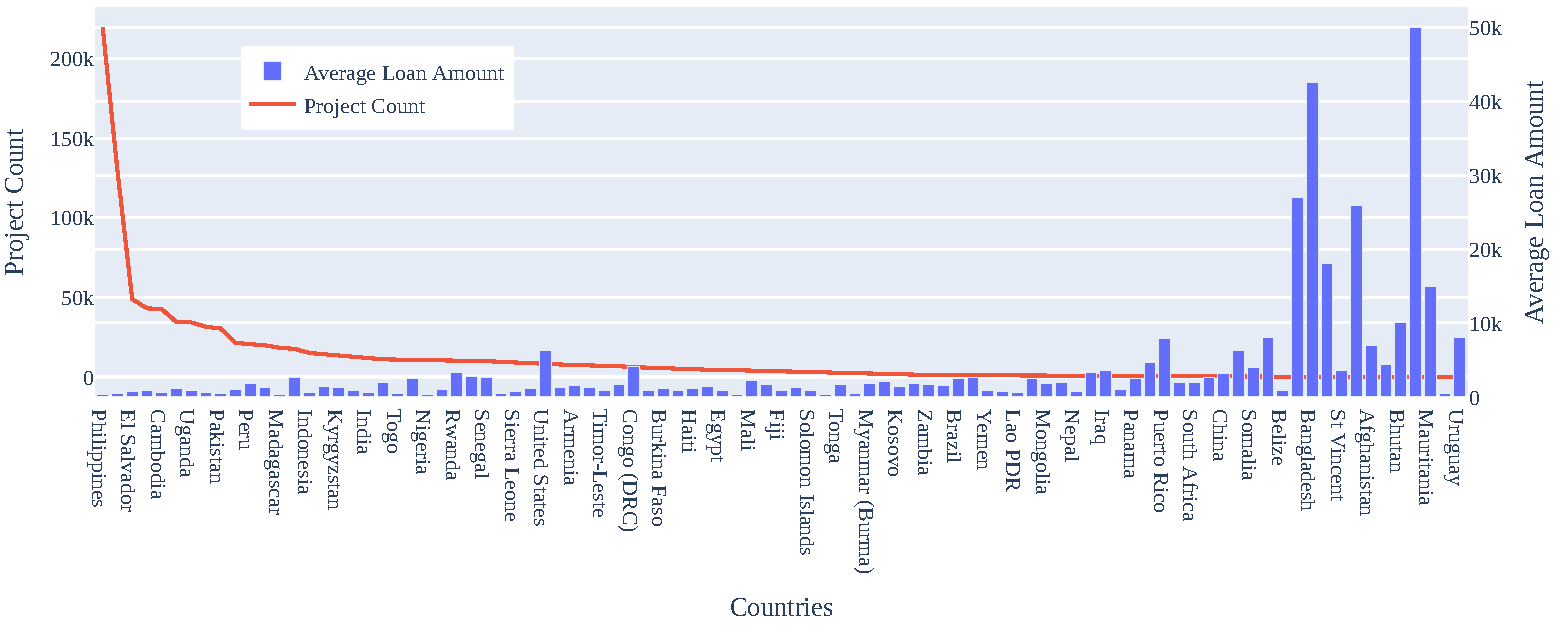
\includegraphics[width=0.95\textwidth]{images/project-vs-country.pdf}
	\caption[Number of Projecst and Average amount of required money for each project by Country]{
		Number of Projecst and Average amount of required money for each project by Country.
		More detail in Table \ref{tab:appendix-project-vs-country}
	}
	\label{fig:country-project-distribution}
\end{figure}


Since the Projects are concentrated in some countries,
and some countries has a higher average amount of money ask by each project,
it will be promising to find community of Lenders who interest in Projects in those countries.


\subsection{Distribution of Projects Across Sectors}

The graph in Figure \ref{fig:project-vs-sector} shows the number of Projects,
as well as the average amount of money asked by each project, by Sector.
We could see that there are some Sectors that have a subtainial large number of Projects, such as Agriculture, Food, Retail, etc.
But when it comes to the average amount of money ask by each project, those Sectors are not the top.
Some Sectors, while limited in the number of Projects, have a large amount of money ask by each project, such as Manufacturing, Wholesale, or Entertainment.

\begin{figure}[H]
	\centering
	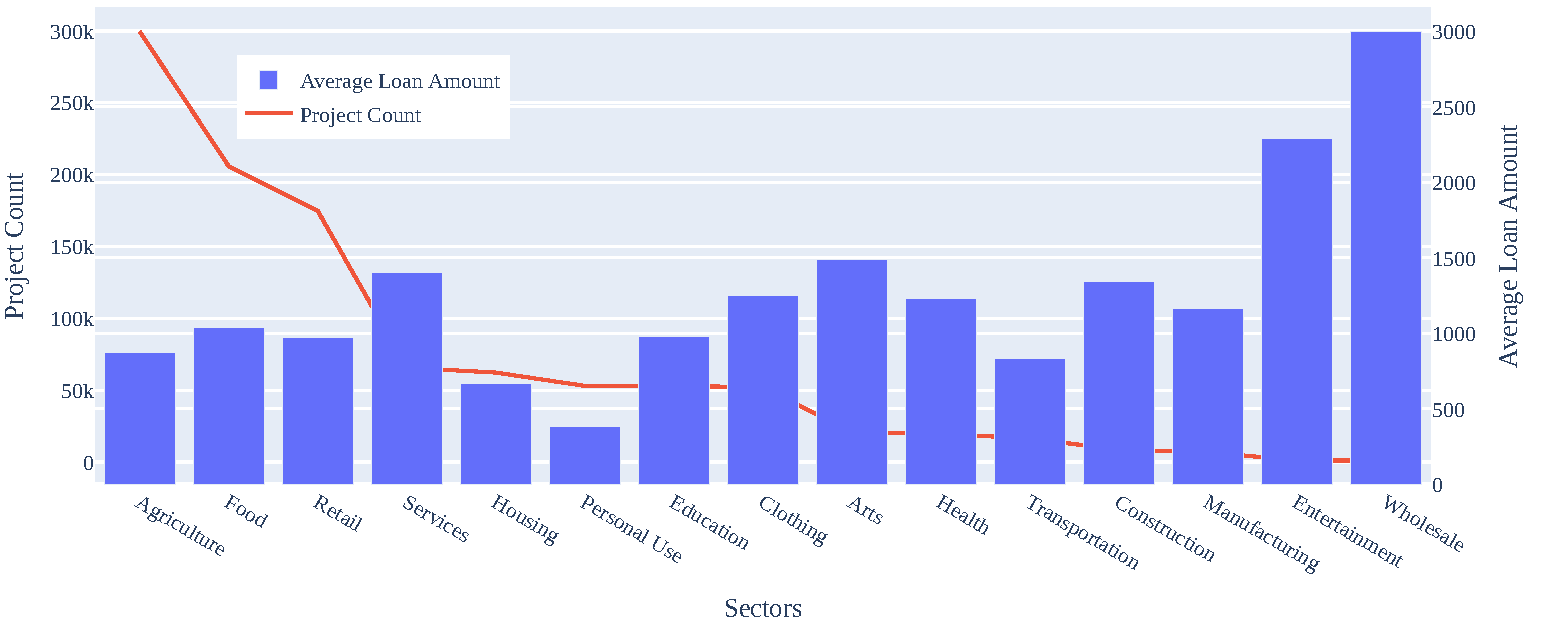
\includegraphics[width=0.8\textwidth]{images/project-vs-sector.pdf}
	\caption{}
	\label{fig:project-vs-sector}
\end{figure}

We could not interpret many meaning from the figure
except that the Sectors are not distributed evenly.
For instance Agriculture usually ask for a smaller amount of money comparing to Services.
Or Personal Use required the least, which is intuitively understandable.
Since the Sectors itself have descriptive meaning and the projects spand accross all the Sectors,
it should not be ignore in the analysis.

\subsection{Distribution of Projects Across Tags}

\todo{continue here}


\begin{figure}[H]
	\centering
	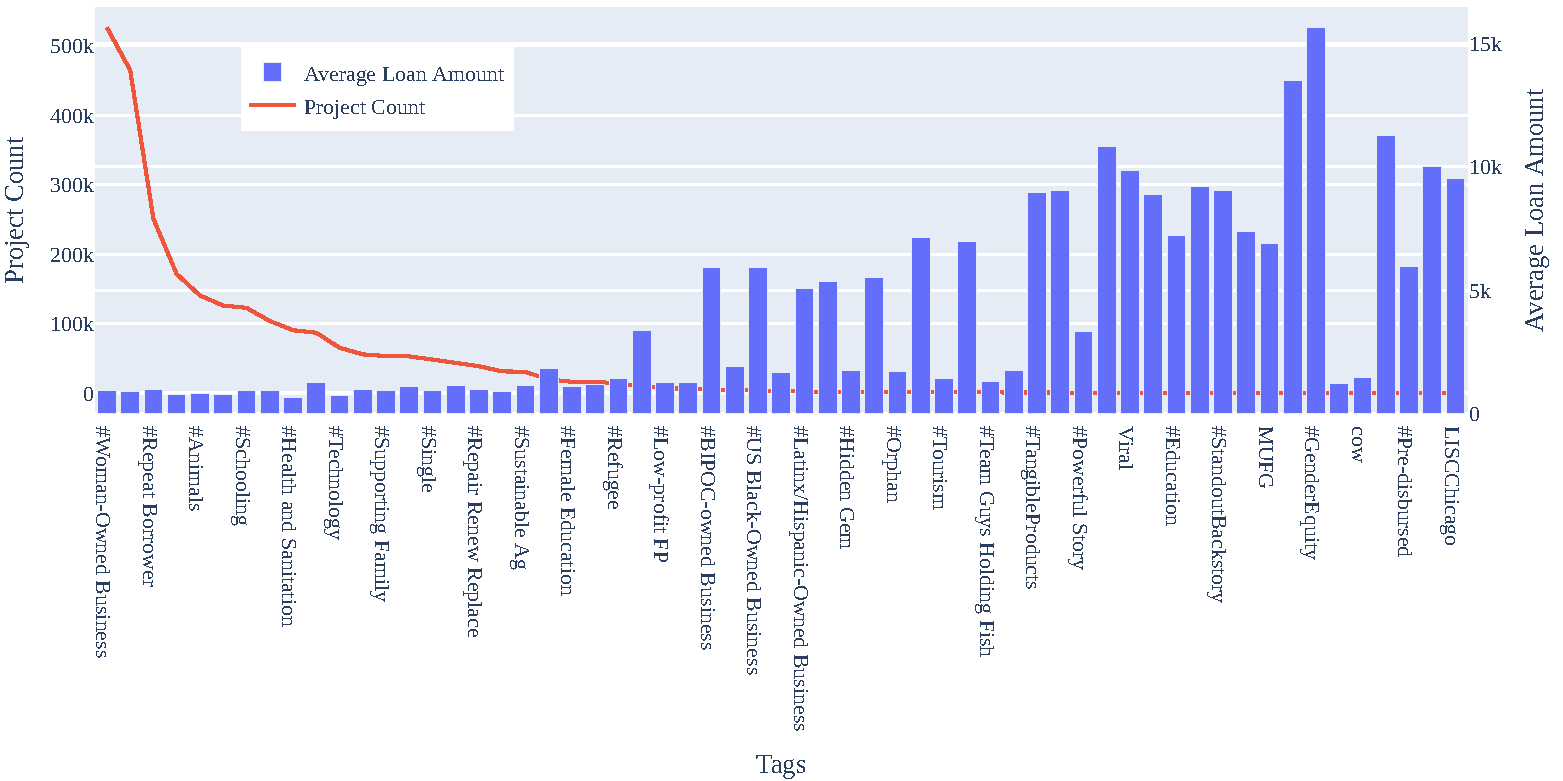
\includegraphics[width=0.8\textwidth]{images/project-vs-tag.pdf}
	\caption{}
	\label{fig:project-vs-tag}
\end{figure}



\todo{tags analysis (the presentation slide)}


While Sector and Country are mandatory fields of a Project, Tags are not.
Recall that we have found that some Tags are used internally by Kiva to manage the data.
In the preprocessing steps, we had removed those Tags.

\todo{Report number project without tags is }

\subsection{How long that users stay on the platform}

Recall that we would like to address if there are community of Lenders in the platform.
We have a hypothesis that, if every lender always give money, and then leaf the platform,
then there are no community of Lenders.
We will try to find out how long that a Lender stay on the platform.

Defined that a Lender is active in a year if he/she give money to a project, which is posted on that year.
We also define that a Lender is active in a range of year if he/she is active in all the years in that range.
Fiture \ref{fig:active-hist} shows the distribution of the number of consecutive years that a Lender is active.
We can see that most of the Lenders are active in only one year.
This is not a good sign for finding community of Lenders.


\begin{figure}[H]
	\centering
	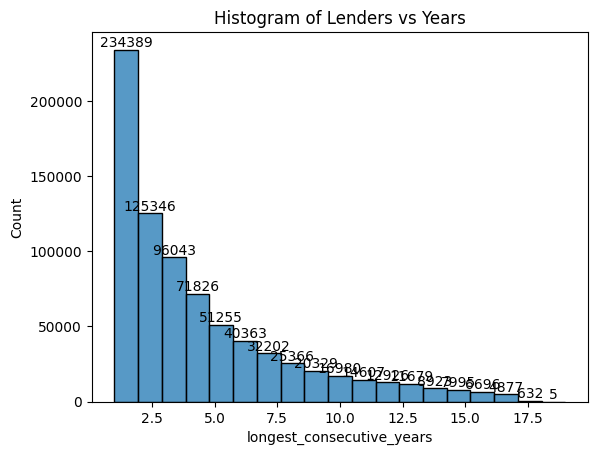
\includegraphics[width=0.8\textwidth]{images/active-hist.png}
	\caption{Number of consecutive years that a Lender funded}
	\label{fig:active-hist}
\end{figure}

We also try to find out the portion of Lenders that are active in a range of years.
To do it, we will construct a table that has following structure.
The y-axes is the start year,
while the x-axes is the end year that we concern.
For each pair of years, we will calculate the \textit{Jaccard index}
between the set of Lenders that are active in that range of years.
For example, if the set of Lender who are active in 2020, 2021, 2022 are
$L_{2020}, L_{2021}, L_{2022}$ respectively,
then the Jaccard index between 2020 and 2022 would be

\begin{equation}
	J(L_{2020}, L_{2021}, L_{2022}) = \frac{|L_{2020} \cap L_{2021} \cap L_{2022}|}{|L_{2020} \cup L_{2021} \cup L_{2022}|}
\end{equation}


Figure \ref{fig:active-fromto} shows the result.
We could see that the portion of Lenders that are active decrease as the range of years increase.
Suppose that the new users are entering the platform and some users also leave the platform,
then this result make sense.


\begin{figure}[H]
	\centering
	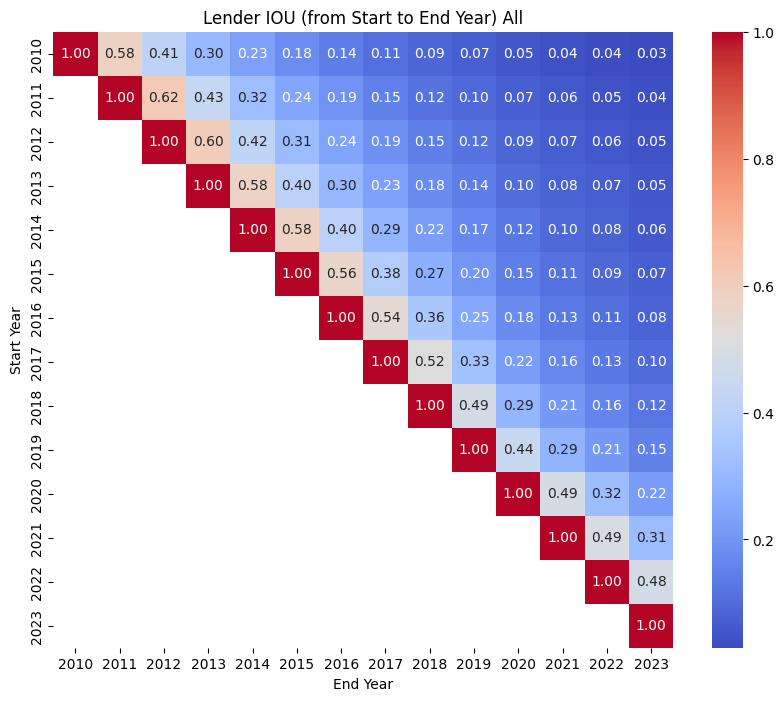
\includegraphics[width=0.8\textwidth]{images/active-fromto.png}
	\caption{}
	\label{fig:active-fromto}
\end{figure}

In order to find a good community of Lenders,
it is intuitively to select only the Lenders who are to a degree active in the platform.
Because if he or she only contribute to a single project,
then their behavior and their interest is not clear.
If he or she repeatedly give money (stay active),
we could find a pattern in their behavior.
In that sense, we will study the active Lenders from 2019 to 2023.
We belive that this range of years provide modern information,
as well as the number of Lender still large enough for analysis.
